\documentclass{beamer}
\usetheme{afm}

\title{Change of Measure and Its Applications}
\course{Advanced Financial Modeling}
\author{\href{mailto:matteo.sani@unisi.it}{Matteo Sani}}

\begin{document}
\begin{frame}[plain]
  \maketitle
\end{frame}

\section{Change of Measure}

\subsection{Numeraires}
\begin{frame}{Numeraires}
  \begin{itemize}
  \item<1-> Since the main issue in pricing theory is to compute
		\begin{equation}
			\Pi_t = \mathbb{E}^{\mathbb{Q}^X}[D(t,T)V_A|\mathcal{F}_t]
			\label{eq:risk_neutral_pricing}
		\end{equation}
  ideally we would like to define a probability measure $\mathbb{Q}^X$ under which the discounted derivative process is a martingale and such that the expectation of the payoff is analytically tractable (i.e. easy to compute).
  \item<1-> The question that arises is: how can we determine such measure $\mathbb{Q}^X$ ?
  \item<2-> The answer is through \textcolor{red}{change of numeraire}.
  \item<3-> A \textcolor{red}{numeraire} is any strictly positive stochastic process $N_t$ that is taken as a unit of reference when pricing an asset $S_t$
    \begin{equation*}
      \tilde{S_t}:=\frac{S_t}{N_t}, \quad t \ge 0
    \end{equation*}
  \end{itemize}
\end{frame}

\begin{frame}{Numeraires}
  \begin{itemize}
  \item We may compute asset values w.r.t. USD, EUR or JPY.
  \item Others might prefer use commodities: 1~oz of gold could be a numeraire.
  \item In any case, once we choose a numerarie e.g. 1 USD, we determine the value of all the other assets:
    \begin{columns}
    	\column{0.5\linewidth}
      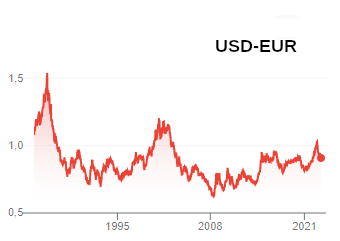
\includegraphics[width=0.9\linewidth]{usd_eur}
    	\column{0.5\linewidth}
      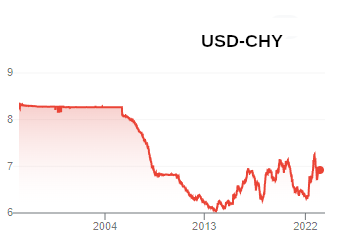
\includegraphics[width=0.9\linewidth]{usd_chy}
    \end{columns}
  \end{itemize}
\end{frame}

\begin{frame}{Numeraires}
  \begin{itemize}
  \item Of course, in practice there are reasons to prefer gold to other commodities e.g. corn, live cattle, or one currency with respect to another (i.e. political reasons)\ldots
  \item But intuitively there should be no theoretical reason (at least at the scale of investors) to prefer to measure value in gold rather than USD (there used to be also the "gold standard")
  \item Basically we want to exploit this fact in our financial models.
  \end{itemize}
\end{frame}

\begin{frame}{Numeraires}
  \begin{itemize}
  \item<1-> \textcolor{red}{Deterministic numeraires} are easy to handle as they imply just an algebraic transformation (i.e. do not involve any risk),
    \begin{itemize}
    \item the exchange rate of the Italian Lira to the Euro was locked at EUR 1 = ITL 1936.27 on 31 December 1998.
    \end{itemize}
  \item<2-> When the numeraire is a \textcolor{red}{stochastic process}, and we want to move to it, the pricing of a claim has to be changed in order to take into account the new risks (the intrinsic randomness of the new numeraire).
  \item<3-> In particular a change of numeraire implies also a change in the underlying measure (probability distribution). Indeed, starting with the bank account numeraire
    \begin{equation*}
      \begin{cases}
        \cfrac{S}{B_t} = \cfrac{\sum_i S_i p_i}{e^{rt}}\\
        \cfrac{U}{B_t} = \cfrac{\sum_i U_i p_i}{e^{rt}}
      \end{cases}\implies
      \frac{S}{U} = \frac{\sum_i S_i p_i}{\sum_j U_j p_j} = \sum_i S_i \frac{p_i}{\sum_j U_j p_j} = \sum_i S_i \pi_i
    \end{equation*}
  \end{itemize}
\end{frame}

\begin{frame}{Numeraire Examples (I)}
  \begin{itemize}
  \item<1-> \textbf{Money market account.} Given $r_t$, a possibly random and time dependent risk-free interest rate process, let
    \begin{equation*}
      B_t := \exp\left(\int_0^t r_s ds\right)
    \end{equation*}
    In this case 
    \begin{equation*}
      \tilde{S_t}:=\frac{S_t}{B_t}=e^{-\int_0^t r_s ds}S_t, \quad t \ge 0
    \end{equation*}
    represents the discounted price of the asset at time 0.
  \item<2-> \textbf{Currency exchange rate.} In this case $N_t := R_t$ denotes e.g. the EUR/SGD exchange rate. Let
    \begin{equation*}
      \tilde{S_t}:=\frac{S_t}{R_t}, \quad t \ge 0
    \end{equation*}
    denotes the price of a local (SG) asset quoted in units of the foreign currency (EUR) (notice the difference with previous ITL/EUR example above).
  \end{itemize}
\end{frame}

\begin{frame}{Numeraire Examples (II)}
  \begin{itemize}
  \item<1-> \textbf{Forward numeraire.} The price $P(t,T)$ of a bond paying $P(T,T)=1$ at maturity $T$. In this case
    \begin{equation*}
      N_t := P(t,T)=\mathbb{E}\left[e^{\int_t^T r_s ds}\right]
    \end{equation*}
    %Notice that the process $t\rightarrow e^{\int_0^t r_s ds} P(t,T)=\mathbb{E}\left[e^{\int_0^T r_s ds}\right], \quad 0 \le t \le T$ is a martingale.
  \item<2-> \textbf{Annuity numeraire.} Processes of the form
    \begin{equation*}
      N_t = P(t, T_0, T_n) := \sum_{k=1}^{n}(T_k - T_{k-1})P(t, T_k), \quad 0 \le t \le T
    \end{equation*}
    where $P(t,T_1),P(t,T_2),\ldots,P(t,T_n)$ are bond prices with maturities $T_1 < T_2 < \ldots < T_n$.
  \end{itemize}
\end{frame}

\subsection{Radon-Nikodym Derivative}
\begin{frame}{Radon-Nikodym Derivative}
  \begin{itemize}
  \item Now we need to understand how to pass from a numeraire to another, and hence by a measure to another, in an arbitrage free setting.
  \item Notice that until now we have implicitly assumed the bank account $B$ as our numeraire.
  \item Before formalize how this passage can be done it is worth stating the following:
  	\begin{itemize}
	  \item Formally we can indicate with
	  \begin{equation*}
	  	\begin{gathered}
	  	\mathbb{N}_\mu := \{A\in \Omega \mid \mu(A)=0\}\\
  	  	\mathbb{N}_\nu := \{A\in \Omega \mid \nu(A)=0\}
  	  \end{gathered}
    \end{equation*}
  	the $\mu$-null sets and the $\nu$-null sets, respectively. 
  	The two measures are called equivalent if and only $\mathbb {N}_\mu= \mathbb{N}_\nu$.
	\item In other words two probability measures are said to be equivalent when they agree on which events have measure zero.
  \end{itemize}
  \end{itemize}
\end{frame}

\begin{frame}{Radon-Nikodym Derivative}
	\begin{block}{Definition}
		When two measures are equivalent it is possible to express the first in terms of the second through the \textcolor{red}{Radon-Nikodym derivative}. Indeed there exists a \textcolor{red}{martingale process $\zeta_t$} such that
		\begin{equation*}
			\mathbb{Q}^* =\int_{A} \zeta_t(\omega)d\mathbb{Q}(\omega)
		\end{equation*}
		which can be written in a more concise form as
		\begin{equation}
			\frac{d\mathbb{Q}^*}{d\mathbb{Q}} = \zeta_t
			\label{eq:radon_nikodym_der}
		\end{equation}
	\end{block}
\end{frame}

\begin{frame}{Intuition from Expected Value}
  \begin{itemize}
  \item To get a sense of what a Radon-Nikodym derivative is we can write the expected value of a generic function $F(x)$ under a measure $\mathbb{P}$, with associated density function $p(x)$ as
    \begin{equation*}
      \expect{P}=\int F(x)p(x)dx
    \end{equation*}
  \item Suppose there exists a function $q(x)$, which satisfies the mathematical conditions required to be a density function. Then we can write
    \begin{equation*}
      \expect{P}=\int F(x)p(x)\frac{q(x)}{q(x)}dx
    \end{equation*}
  \item If we define $\psi(x)=F(x)\frac{p(x)}{q(x)}$ the expected value can be written as 
    \begin{equation*}
      \expect{P}[F(x)]=\int\psi(x)q(x)dx=\expect{Q}[\psi(x)]=\expect{Q}\left[F(x)\frac{p(x)}{q(x)}\right]
    \end{equation*}
  \end{itemize}
\end{frame}

\begin{frame}{Radon-Nikodym Derivative}
  \begin{itemize}
  \item The expectations corresponding to the two measures are related by
    \begin{equation*}
      \expect{Q^*}[X] = \expect{Q}\left[X\frac{d\mathbb{Q}^*}{d\mathbb{Q}}\right]= \expect{Q}[X\zeta]
    \end{equation*}
	\pause
  \item In case of a conditioned expectation
    \begin{equation}
      \expect{*}[X|\mathcal{F}_t] = \frac{\mathbb{E}\left[X\cfrac{d\mathbb{Q}^*}{d\mathbb{Q}}\bigg|\mathcal{F}_t\right]}{\mathbb{E}[\zeta_t|\mathcal{F}_t]}
      \label{eq:conditioned_expectation}
    \end{equation}
    which is an "equivalent" formulation of the famous \emph{Bayes theorem}
    \begin{equation*}
      P(A|B)=\frac{P(B|A)P(A)}{P(B)}
    \end{equation*}
  \end{itemize}
\end{frame}

\begin{frame}[fragile]{Radon-Nikodym Derivative Example}
  \begin{itemize}
      \item Imagine two probability densities $\mathbb{P} = \mathcal{N}(\mu_1, \sigma_1)$ and $\mathbb{Q} = \mathcal{N}(\mu_2, \sigma_2)$.
      \item Let's numerically compute the Radon-Nikodym derivative the moves you from the $\mathbb{P}$ to the $\mathbb{Q}$ world.
  \end{itemize}

\codebox{code/radon_nikodym_ex}
\end{frame}

\begin{frame}[fragile]{Radon-Nikodym Derivative Example}
\begin{center}
    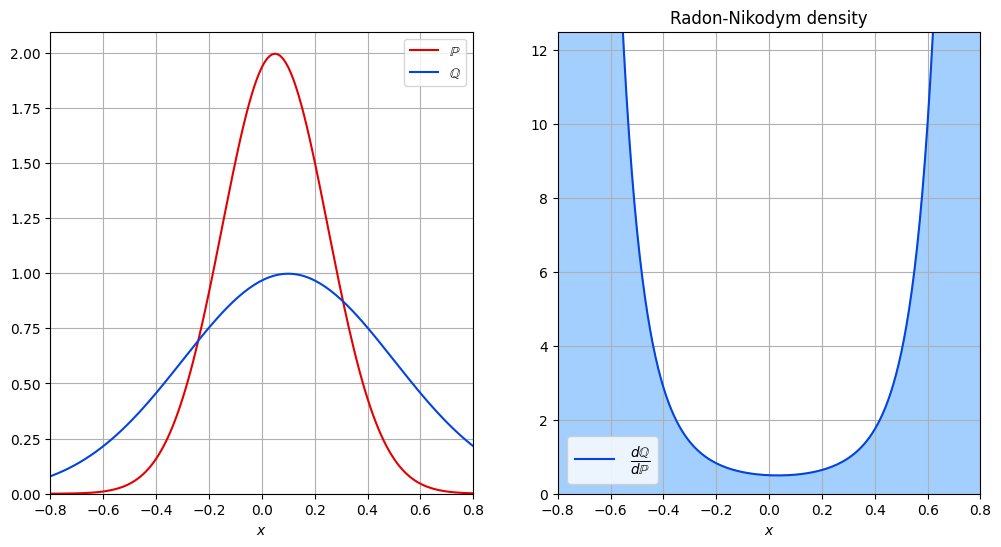
\includegraphics[width=0.9\linewidth]{images/radon_nikodym_plot}
\end{center}
\end{frame}

\begin{frame}[fragile]{Radon-Nikodym Derivative Example}
\begin{itemize}
    \item Consider Consider the Radon-Nikodym derivative
\begin{equation*}
\cfrac{d\mathbb{Q}}{d\mathbb{P}}=\zeta;\quad Q(A) = \int_A \zeta dP
\end{equation*}
    \item What is $\mathbb{E}[\zeta]$ ? Intuitively, we have that
\begin{equation*}
\mathbb{E}[\zeta]=\mathbb{E}\left[\frac{dQ}{dP}\right]=\int \frac{dQ}{dP} dP
\end{equation*}
so the $dP$ "cancel out" and we get
\begin{equation*}
\mathbb{E}[\zeta]=\int dQ = 1
\end{equation*}
\end{itemize}
\end{frame}

\begin{frame}[fragile]{Radon-Nikodym Derivative Example}
\begin{columns}
\column{0.5\linewidth}
    Let's verify our calculation with a Monte Carlo simulation:
    \begin{equation*}
        \begin{gathered}
        <f(x)> = \frac{1}{b-a}  \int_{a}^{b} f(x) \,dx\\
        \int_{a}^{b} f(x) \,dx = (b-a) <f(x)>\\
        \int_{a}^{b} f(x) \,dx \approx (b-a) \frac{1}{N} \sum_{i=1}^{N} f(x_i)
        \end{gathered}
    \end{equation*}
\column{0.5\linewidth}
\codebox{1\linewidth}{code/radon_nikodym_expectation}
\outputbox{1\linewidth}{code/radon_nikodym_expectation}
\end{columns}
\end{frame}














%\begin{frame}{Conditional Expectation}
%	\begin{itemize}
%	\item The classic form of Bayes' theorem for continuous random variables involves integrating over the parameter space:
%	\begin{equation*}	
%	P(\theta|x) = \cfrac{p(x|\theta)P(\theta)}{\int p(x|\theta')P(\theta')d\theta'}
%	\end{equation*}
%	\item Now, introduce a reference probability density function $q(x)$ on the same data space as $p(x)$. The Radon-Nikodym derivative is such that:
%	\begin{equation*}
%	\int f(x)q(x)dx = \int p(x)dx
%	\end{equation*}
%	\item In our case, we can choose $q(x)$ to be the marginal density $P(x)$. Then, the likelihood function in Bayes' theorem can be represented using the Radon-Nikodym derivative:
%	\begin{equation*}
%	P(\theta|x) = d(p(x|\theta)P(\theta)|P(x))
%	\end{equation*}
%	\item This means the posterior density of the parameter $\theta$ given the data $x$ is proportional to the Radon-Nikodym derivative of the product of the likelihood function and the prior density, with respect to the marginal density.
%	\item Intuitively, the Radon-Nikodym derivative measures how much "denser" the product of the likelihood and prior is compared to the marginal density at each data point $x$. This "rate of change" helps identify parameter values that make the observed data more likely, updating our belief about the parameter based on the evidence.
%	\end{itemize}	
%\end{frame}

\subsection{Change of Numeraire}
\begin{frame}{Change of Numeraire}
  \begin{block}{Theorem}
  	\small{
    Assume exists a numeraire $N_t$ and the associated measure $\mathbb{Q}^N$, equivalent to $\mathbb{P}$, such that the price of any traded asset $S_t$ relative to $N$ is a martingale under $\mathbb{Q}^N$
    \begin{equation*}
      \frac{S_t}{N_t} = \expect{N}\left[\frac{S_T}{N_T}\bigg|\mathcal{F}_t\right],\quad 0\le t \le T
    \end{equation*}
    Let $U$ be another arbitrary numeraire. Then there exists a measure $\mathbb{Q}^U$, also equivalent to $\mathbb{P}$, such that the price of any traded asset $S_t$, normalized to $U$, is a martingale under $\mathbb{Q}^U$
    \begin{equation*}
      \frac{S_t}{U_t} = \expect{U}\left[\frac{S_T}{U_T}\bigg|\mathcal{F}_t\right],\quad 0\le t \le T
    \end{equation*}
    The Radon-Nikodym derivative defining the measure $\mathbb{Q}^U$ is given by
\begin{equation}
	\frac{d\mathbb{Q}^U}{d\mathbb{Q}^N} = \frac{U_T N_0}{U_0 N_T}
	\label{eq:radon_nikodym_der2}
\end{equation}}
  \end{block}
\end{frame}	

\begin{frame}{Change of Numeraire (Proof part 2)}
	\begin{itemize}
		\item Let's prove first this second part.
  		\item By definition of $\mathbb{Q}^N$, for any asset price $S_t$ holds
	  \begin{equation*}
	    \begin{cases} 
	      \expectt{N}{t}\left[\cfrac{S_T}{N_T}\right] = \cfrac{S_0}{N_0} \\
\expectt{U}{t}\left[\cfrac{U_0 S_T}{N_0 U_T}\right] = \cfrac{U_0}{N_0}\expectt{U}{t}\left[\cfrac{S_T}{U_T}\right] = \cfrac{\cancel{U_0} S_0}{N_0 \cancel{U_0}} = \cfrac{S_0}{N_0}
	    \end{cases}
	  \end{equation*}
  	\item Since both equations result to $S_0/N_0$ they can be equated
  	\begin{equation*}
  	\expectt{N}{t}\left[\cfrac{S_T}{N_T}\right] = \expectt{U}{t}\left[\cfrac{U_0 S_T}{N_0 U_T}\right]
  	\end{equation*}
  	\end{itemize} 
\end{frame}

\begin{frame}{Change of Numeraire (Proof part 2)}
	\begin{itemize}
	\item By definition of Radon-Nikodym derivative and from the result of in previous slide, it holds
  \begin{equation*}
  	\begin{cases}
    \expectt{N}{t}\left[\cfrac{S_T}{N_T}\right] =\expectt{U}{t}\left[\cfrac{S_T}{N_T} \cfrac{d\mathbb{Q}^N}{d\mathbb{Q}^U}\right] \\
    \expectt{N}{t}\left[\cfrac{S_T}{N_T}\right] =\expectt{U}{t}\left[\cfrac{U_0 S_T}{N_0 U_T}\right]
    \end{cases}\implies
	\cfrac{\cancel{S_T}}{N_T} \cfrac{d\mathbb{Q}^N}{d\mathbb{Q}^U} = \cfrac{U_0 \cancel{S_T}}{N_0 U_T}
  \end{equation*}
	where we have used the fact that the expectation arguments under $U$ must equal to get \cref{eq:radon_nikodym_der2}. 
  \end{itemize}
\myendproof
\end{frame}

\begin{frame}{Change of Numeraire (Proof part 1)}
  \begin{itemize}
  \item<1-> Now we can prove the first part of the change of numeraire theorem. The conditional expectation formula~\cref{eq:conditioned_expectation} gives
    \begin{equation*}
      \expect{U}\left[\cfrac{S_T}{U_T}\bigg|\mathcal{F}_t\right]=\cfrac{\expect{N}\left[\cfrac{d\mathbb{Q}^U}{d\mathbb{Q}^N}\cfrac{S_T}{U_T}\bigg|\mathcal{F}_t\right]}{\expect{N}\left[\cfrac{d\mathbb{Q}^U}{d\mathbb{Q}^N}\bigg|\mathcal{F}_t\right]}
    \end{equation*}
  \item<2-> But 
    \begin{equation*}
      \begin{cases}
	\expectt{N}{t}\left[\cfrac{d\mathbb{Q}^U}{d\mathbb{Q}^N}\cfrac{S_T}{U_T}\right]= \expectt{N}{t}\left[\cfrac{\cancel{U_T} N_0}{N_T U_0}\cfrac{S_T}{\cancel{U_T}}\right]=\cfrac{N_0 S_t}{U_0 N_t} \\
	\expectt{N}{t}\left[\cfrac{d\mathbb{Q}^U}{d\mathbb{Q}^N}\right]= \expectt{N}{t}\left[\cfrac{U_T N_0}{N_T U_0}\right] = \cfrac{N_0 U_t}{U_0 N_t}\quad\text{(the RND is a martingale)}
      \end{cases}
    \end{equation*}
  \end{itemize}
\end{frame}	

\begin{frame}{Change of Numeraire (Proof part 1)}
	\begin{itemize}
		\item Now we can prove the first part of the change of numeraire theorem. The conditional expectation formula~\cref{eq:conditioned_expectation} gives
		\begin{equation*}
			\expect{U}\left[\cfrac{S_T}{U_T}\bigg|\mathcal{F}_t\right]=\cfrac{\expect{N}\left[\cfrac{d\mathbb{Q}^U}{d\mathbb{Q}^N}\cfrac{S_T}{U_T}\bigg|\mathcal{F}_t\right]}{\expect{N}\left[\cfrac{d\mathbb{Q}^U}{d\mathbb{Q}^N}\bigg|\mathcal{F}_t\right]} = \cfrac{\cfrac{\cancel{N_0} S_t}{\cancel{U_0} \cancel{N_t}}}{\cfrac{\cancel{N_0} U_t}{\cancel{U_0} \cancel{N_t}}} = \cfrac{S_t}{U_t}
		\end{equation*}
		\item But 
		\begin{equation*}
			\begin{cases}
				\expectt{N}{t}\left[\cfrac{d\mathbb{Q}^U}{d\mathbb{Q}^N}\cfrac{S_T}{U_T}\right]= \expectt{N}{t}\left[\cfrac{\cancel{U_T} N_0}{N_T U_0}\cfrac{S_T}{\cancel{U_T}}\right]=\cfrac{N_0 S_t}{U_0 N_t} \\
				\expectt{N}{t}\left[\cfrac{d\mathbb{Q}^U}{d\mathbb{Q}^N}\right]= \expectt{N}{t}\left[\cfrac{U_T N_0}{N_T U_0}\right] = \cfrac{N_0 U_t}{U_0 N_t}
			\end{cases}
		\end{equation*}
	\end{itemize}
\myendproof
\end{frame}	

\begin{frame}{Change of Numeraire Remarks}
  This powerful theorem, we have just proved allows to
\begin{enumerate}
    \item find a characterization of our process by means of which we can work-out more easily the fundamental pricing formula. In particular allows to find a measure associated to the new numeraire such that \textcolor{red}{the price of any asset divided by that numeraire is a martingale};
    \item give a simple rule to write (the otherwise difficult to derive) Radon-Nikodym derivative;
      \item \textcolor{red}{the risk-neutral price is invariant under change of numeraire}
    \begin{equation*}
    	\text{Price} = \expectt{N}{t}\left[\cfrac{N_0 S_T}{N_T}\right] = \expectt{U}{t}\left[\cfrac{U_0 S_T}{U_T}\right]
    \end{equation*}
    \end{enumerate}
\end{frame}

\begin{frame}{Asset Price divided by Numeraire}
	\begin{itemize}
 	\item<1-> Let $B$ be the money bank numeraire and $\mathbb{Q}^B$ the corresponding risk-neutral measure. Also let $N$ be another numeraire (note that for what just said $N/B$ is a $\mathbb{Q}^B$-martingale). 
	\item<2-> From the Change of Numeraire Theorem we can define a new measure by mean of
  \begin{equation*}
    \frac{d\mathbb{Q}^N}{d\mathbb{Q}^B} = \frac{N_TB_0}{B_TN_0}
  \end{equation*}
	\item<3-> Then, for any asset $S$ such that $S/B$ is a $\mathbb{Q}^B$-martingale
  \begin{equation*}
    \expect{N}\left[\frac{S_T}{N_T}\bigg|\mathcal{F}_t\right] = \cfrac{\expect{B}\left[\cfrac{S_T}{N_T}\cfrac{N_TB_0}{B_TN_0}\bigg|\mathcal{F}_t\right]}{\expect{B}\left[\cfrac{N_TB_0}{B_TN_0}\bigg|\mathcal{F}_t\right]}
    =\cfrac{\expect{B}\left[\cfrac{S_T}{B_T}\bigg|\mathcal{F}_t\right]}
    {\expect{B}\left[\cfrac{N_T}{B_T}\bigg|\mathcal{F}_t\right]}
    =\frac{S_tB_t}{N_tB_t}=\frac{S_t}{N_t}
  \end{equation*}
\myendproof
	\item<4-> \textcolor{red}{So $S/N$ is a $\mathbb{Q}^N$-martingale.}
	\end{itemize}
\end{frame}

\subsection{Applications}
\begin{frame}{Examples}
  \footnotesize{\tiny {\tiny }}{
    \begin{table}[bt]
      \renewcommand*{\arraystretch}{1.4}
      \begin{tabular}{|l|l|} \hline
	\begin{tabular}{@{}l@{}}
	  Any asset divided by the bank account
	  $B_t$\\(recall $dB_t = r_t B_t dt$)
	  \boxed{\cfrac{S_t}{B_t} = e^{-\int_0^t r_s ds}S_t}
	\end{tabular}
	& \begin{tabular}{l}
	    It is a martingale under the\\
	    measure $\mathbb{Q}^B$ associated to \\
	    the bank account numeraire,\\
  	    i.e. the risk neutral measure.
	  \end{tabular} \\ \hline
	\begin{tabular}{@{}l@{}}
	  The forward rate\\
	  \boxed{F(t; T_1, T_2) = \frac{1}{T_2-T_1}\left(\frac{P(t,T_1) - P(t,T_2)}{P(t,T_2)}\right)}\\
	  can be interpreted as a portfolio of two ZCBs\\
	  divided by another ZCB.		
	\end{tabular}
	& \begin{tabular}{l}
	    Under the measure $\mathbb{Q}^2$\\ 
	    associated to the numeraire\\ 
	    $P(\cdot,T_2)$ it is a martingale.\end{tabular}\\ \hline  
	\begin{tabular}{@{}l@{}}
	  The swap rate
	  \boxed{S_{\alpha,\beta}(t) = \frac{P(t,T_\alpha)-P(t,T_\beta)}{\sum_{i=\alpha+1}^{\beta}\tau_i P(t,T_i)}}
	  \\can be interpreted as a portfolio of two ZCBs\\
	  divided by a portfolio of ZCBs.		
	\end{tabular}
	& \begin{tabular}{l}
	    It is a martingale under the\\
	    measure associated to the\\
	    annuity numeraire.
	  \end{tabular} \\ \hline
      \end{tabular}
  \end{table}}
\end{frame}

\begin{frame}{A Useful Separation}
  \begin{itemize}
  \item<1-> Until now we have used $B(t)$, the money market account, as numeraire. But as we have seen it is natural to look for the most convenient one, that is, the one which minimizes the mathematical difficulties according to the problem at hand.
  \item<2-> Given a contingent claim whose payoff at time $T$ is $\chi$, we have the following formula for its price $\Pi$
    \begin{equation*}
      \Pi_\chi(t,T)=\expect{B}\left[e^{-\int_t^T r_s ds}\chi\bigg|\mathcal{F}_t \right]=\expect{B}\left[e^{\int_0^t r_s ds}e^{-\int_0^T r_s ds}\chi\bigg|\mathcal{F}_t \right]=B_t\expect{B}\left[B^{-1}_T\chi|\mathcal{F}_t\right]
    \end{equation*}
  \item<3-> If $\chi$ and the short rate process were independent under $\mathbb{Q}^B$ (recall $\mathbb{E}[XY]=\mathbb{E}[X]\mathbb{E}[Y]$) then we could write
    \begin{equation*}
      \Pi_\chi(t,T)=\expect{B}\left[e^{-\int_t^T r_s ds}\bigg|\mathcal{F}_t\right]\expect{B}\left[\chi|\mathcal{F}_t\right] = P(t,T)\expect{B}\left[\chi|\mathcal{F}_t\right]
    \end{equation*}
  \end{itemize}
\end{frame}

\begin{frame}{A Useful Separation}
  \begin{itemize}
  \item<1-> In general the above separation is not possible due to the interaction between the discount factors and the claim payoff. 
  \item<2-> In this, like in other concrete situations, a better numeraire is indeed the ZCB with the same maturity $T$ of the derivative to price (recall $P(T,T)=1)$.
  \item<3-> The \textcolor{red}{forward measure $\mathbb{Q}^T$ (also called the $T$-measure)} is defined as the martingale measure for the numeraire process $P(\cdot,T)$, the ZCB maturing in T indeed, i.e. what we called $\mathbb{Q}^2$ in the example above.
  \item<4-> It is easy to see that using \cref{eq:radon_nikodym_der2}, the Radon-Nykodim derivative is given in this case by
    \begin{equation}
      \zeta_t = \frac{d\mathbb{Q}^T}{d\mathbb{Q}^B} = \frac{P(t,T)\overbrace{B(0)}^{=1}}{B_t P(0,T)} ,\quad\left(\zeta_T=\frac{\overbrace{P(T,T)}^{=1}B(0)}{B(T)P(0,T)}=\frac{1}{B(T)P(0,T)}\right)
      \label{eq:radon_nikodym_t_forward}
    \end{equation}
  \end{itemize}
\end{frame}

\begin{frame}{A Useful Separation}
  \begin{itemize}
  \item<1-> Applying the change of numeraire to the pricing formula, we get
    \begin{equation*}
      \begin{aligned}
	\Pi_\chi(t,T) & = B_t\expect{B}\left[B^{-1}_T\chi|\mathcal{F}_t\right] \\
	& = B_t\expect{B}\left[P(0,T)\zeta_T\chi|\mathcal{F}_t\right]\quad\text{(using } B_T^{-1} = \zeta_TP(0,T))\\
	& = B_tP(0,T)\expect{B}\left[\zeta_T|\mathcal{F}_t\right]\expect{T}\left[\chi|\mathcal{F}_t\right]\text{(by \cref{eq:conditioned_expectation}, cond. expect.)}\\
	& = B_tP(0,T)\zeta_t\expect{T}\left[\chi|\mathcal{F}_t\right] =  \cancel{B_tP(0,T)}\frac{P(t,T)}{\cancel{B_tP(0,T)}}\expect{T}\left[\chi|\mathcal{F}_t\right] \\
	& = P(t,T)\expect{T}\left[\chi|\mathcal{F}_t\right] \\
      \end{aligned}
    \end{equation*}
    which achieves the desired separation (although under a new measure).
  \item<2-> Clearly this kind of transformation is useful when $\chi$ has known dynamics under the forward measure.
  \end{itemize}
\end{frame}

\begin{frame}{Identity between $\mathbb{Q}^B$ and $\mathbb{Q}^T$}
  By construction of the martingale measure $\mathbb{Q}^B$, the following relationship holds
  \begin{equation*}
    \begin{gathered}
      \frac{P(t,T)}{B_t}=\expect{B}\left[\frac{P(T,T)}{B_T}\right]\\[0.3cm]
      P(t,T)=\expect{B}\left[\frac{P(T,T)}{B_T}B_t\right] = \expect{B}\left[\frac{B_t}{B_T}\right]
    \end{gathered}
  \end{equation*}
	\pause
  Plugging the result into the Radon-Nikodym derivative gives
  \begin{equation*}
    \frac{d\mathbb{Q}^T}{d\mathbb{Q}^B} = \frac{B_t}{B_T}\frac{1}{P(t,T)} =\frac{B_t/B_T}{\expect{B}[B_t/B_T]}
  \end{equation*}
\myendproof
	\pause
  \begin{block}{Proposition}
    If interest rates are deterministic (i.e. the Radon-Nikodym derivative is 1), then the measures $\mathbb{Q}^B$ and $\mathbb{Q}^T$ are identical.
  \end{block}
\end{frame}

\begin{frame}{Clarification on Time}
  \begin{itemize}
  \item Clearly as the Radon-Nikodym derivative is a martingale for valuation time $t$, we have
    \begin{equation*}
      \frac{d\mathbb{Q}^U}{d\mathbb{Q}^N}=\frac{U_tN_0}{U_0N_t}
    \end{equation*}
  \item Do not confuse the maturity of the numeraire bond $T$ with the times at which you have to take the values of the numeraire, in this case $t$ and 0.
  \item If you want to switch from the $T$ measure to the $S$ measure, i.e. the one induced by the bond $P(.,S)$, for the valuation time $t$ we get
    \begin{equation*}
      \frac{d\mathbb{Q}^S}{d\mathbb{Q}^T}=\frac{P(t,S)P(0,T)}{P(t,T)P(0,S)}
    \end{equation*}
  \end{itemize}
\end{frame}

%%%%%%%%%%%%%%%%%%%%%%%%%%  PARTE 1

\begin{frame}{The Forward Rate Under $\mathbb{Q}^T$}
  \begin{block}{Proposition}
    Consider the forward numeraire $P(t,T)$ and denote with $\mathbb{Q}^T$ its associated measure.
    The forward rate spanning the interval $[S,T]$ is the $\mathbb{Q}^T$-expectation of the future spot rate at time $S$ for the maturity $T$
    \begin{equation}
      F(t;S,T) =\expect{T}[L(S,T)|\mathcal{F}_t]
    \end{equation}
  \end{block}
\end{frame}

\begin{frame}{The Forward Rate Under $\mathbb{Q}^T$ (Proof)}
  \begin{equation*}
    \begin{gathered}
      F(t;S,T) = \frac{1}{\tau}\left[\frac{P(t,S)-P(t,T)}{P(t,T)}\right] \\[0.3cm]
      F(t;S,T)P(t,T) = \frac{P(t,S)-P(t,T)}{\tau}
    \end{gathered}
  \end{equation*}

  This is the price at time $t$ of an asset (difference of two bonds). Therefore by the change of numeraire theorem and by definition of forward measure
  \begin{equation*}
	F(t,S,T) = \frac{F(t;S,T)P(t,T)}{P(t,T)}
  \end{equation*}
  is a \textcolor{red}{martingale} under $\mathbb{Q}^T$-measure. \pause Hence
  \begin{equation*}
    F(t;S,T) = \expect{T}[F(S;S,T)|\mathcal{F}_t] = \expect{T}\left[\frac{1}{\tau}\left(\frac{1-P(S,T)}{P(S,T)}\right)\bigg|\mathcal{F}_t\right] = \expect{T}[L(S,T)|\mathcal{F}_t]
  \end{equation*}
\myendproof
\end{frame}

\begin{frame}{The Forward Rate Under $\mathbb{Q}^T$}
  A similar result can be derived for the corresponding instantaneous quantities
  \begin{equation}
    f(t,T)=\expect{T}[r_t|\mathcal{F}_t]
  \end{equation}
	\pause
  Indeed from the definition of $\mathbb{Q}^B$
  \begin{equation*}
    \frac{P(t,T)}{B_t}=\expect{B}\left[\frac{P(T,T)}{B_T}\bigg|\mathcal{F}_t\right]
  \end{equation*}
  but $P(T,T)=1$ so
  \begin{equation*}
    P(t,T)=\expect{B}\left[\frac{B_tP(T,T)}{B_T}\bigg|\mathcal{F}_t\right]=\expect{B}\left[e^{-\int_t^Tr_u du}\big|\mathcal{F}_t\right]
  \end{equation*}
	\pause
  Differentiating with respect to $T$ ($\frac{d}{dx}\int_c^x f(t)dt=f(x)$)
  \begin{equation*}
    \frac{\partial P(t,T)}{\partial T}=
    \expect{B}\left[-r(T)e^{-\int_t^Tr_u du}\big|\mathcal{F}_t\right]
  \end{equation*}
\end{frame}

\begin{frame}{The Forward Rate Under $\mathbb{Q}^T$}
  Now we can change numeraire to $P(\cdot,T)$ so that, using reciprocal of \cref{eq:radon_nikodym_t_forward} ($\zeta^{-1}=\frac{B_t/B_T}{P(t,T)/P(T,T)}$)
  \begin{equation*}
    \frac{\partial P(t,T)}{\partial T}=
    \expect{T}\left[-r(T)\cancel{e^{-\int_t^Tr_u du}}\frac{P(t,T)}{\cancel{e^{-\int_t^Tr_u du}}}\bigg|\mathcal{F}_t\right]=
    P(t,T)\expect{T}\left[-r(T)|\mathcal{F}_t\right]
  \end{equation*}
	\pause
  Hence
  \begin{equation*}
    \begin{aligned}
      f(t,T)&=\frac{1}{P(t,T)}\frac{\partial P(t,T)}{\partial T}=
      -\frac{\partial \ln P(t,T)}{\partial T}
      = \expect{T}\left[r(T)|\mathcal{F}_t\right]=	\expect{T}\left[f(T,T)|\mathcal{F}_t\right]
    \end{aligned}
  \end{equation*}\myendproof

  Which demonstrates the initial statement and also shows that \textcolor{red}{the instantaneous forward rate is a martingale under the $T$-forward measure}.
\end{frame}

\begin{frame}{The Expectation Hypothesis}
	\begin{itemize}
		\item Previous result
		\begin{equation*}
			f(t, T) = \expect{T}[r(T)|\mathcal{F}_t]
		\end{equation*}
		has a nice connection with the \textcolor{red}{expectation hypothesis of the term structure of interest rates}.
		\item Its basic idea is that the long-term rate is determined purely by current and future expected short-term rates.
		\item We cannot dive into it, but there are a lot of papers on the subject, among which I suggest
		\begin{itemize}
			\item \href{https://pages.stern.nyu.edu/~sternfin/asangvin/ExpHyp.pdf}{\emph{The Expectation Hypothesis, A. Sangvinatsos}}
			\item \href{https://www.jstor.org/stable/2327547}{\emph{A Re-Examination of Traditional Hypotheses about the Term Structure of Interest Rates}, J.C. Cox, J.E. Ingersoll, and S.A. Ross}
			%\item \href{https://www.albany.edu/~bd445/Economics_802_Financial_Economics_Slides_Fall_2013/Risk_Neutrality_and_the_Expectations_Theory.pdf}{\emph{Slides from Fall 2013}}
		\end{itemize}
	%\item According to the pure expectation hypothesis, the above formula is valid if the expected value is taken under the real probability.
	%\item Absence of arbitrage makes this incompatible with stochastic interest rates.
	\end{itemize}
\end{frame}

\begin{homework}
	\begin{frame}{\textcolor{white}{Homework}}
\begin{itemize}
	\item[white] If the pure expectations hypothesis holds, why might the yield curve be flat, upward sloping, or downward sloping? The government implements a credible “tight” monetary policy by raising short-term (e.g. 3-month) interest rates. How could this affect the yield curve?
\end{itemize}
\end{frame}
\end{homework}

%The Relationship between Forward Rate over Second Year
%and Spot Rate Expected over Second Year
%Given a forecast of bond B’s price, an investor can choose one of two strategies at date 0:
% 1. Buy a one-year bond. Proceeds at date 1 would be:
% $1,080 = $1,000 x 1.08 (A.10)

% 2. Buy a two-year bond but sell at date 1. Expected proceeds would be:
% $1,000 x (1.10)2
%____________________________
%1 +  Spot rate expected over year 2 (A.11)
% Given our discussion of forward rates, we can rewrite Equation A.11 as:
% $1,000 x 1.08 x 1.1204
%____________________________
%1  Spot rate expected over year 2 (A.12)
% (Remember that 12.04 percent was the forward rate over year 2; that is, f2 = 12.04%.)
% Under what condition will the return from strategy 1 equal the expected return from
%strategy 2? In other words, under what condition will Equation A.10 equal Equation A.12?
% The two strategies will yield the same expected return only when:
% 12.04%  Spot rate expected over year 2 (A.13)
%In other words, if the forward rate equals the expected spot rate, one would expect to earn
%the same return over the first year whether one
%• Invested in a one-year bond.
%• Invested in a two-year bond but sold after one year.


%The Expectations Hypothesis
%Equation A.13 seems fairly reasonable. That is, it is reasonable that investors would set
%interest rates in such a way that the forward rate would equal the spot rate expected by the
%marketplace a year from now.
% For example, imagine that individuals in the marketplace do
%not concern themselves with risk. If the forward rate, f2, is less than the spot rate expected
%over year 2, individuals desiring to invest for one year would always buy a one-year bond.
%That is, our work shows that an individual investing in a two-year bond but planning to sell
%at the end of one year would expect to earn less than if he simply bought a one-year bond.
% Equation A.13 was stated for the specific case where the forward rate was 12.04 percent.
%We can generalize this as follows:
%Expectations Hypothesis:
% f2 = Spot rate expected over year 2 (A.14)
%Equation A.14 says that the forward rate over the second year is set to the spot rate that
%people expect to prevail over the second year. This is called the expectations hypothesis. It
%states that investors will set interest rates such that the forward rate over the second year is
%equal to the one-year spot rate expected over the second year.


%Liquidity Preference Hypothesis
%At this point, many students think that Equation A.14 must hold. However, note that we
%developed Equation A.14 by assuming that investors were risk-neutral. Suppose, alternatively, that investors are averse to risk.
% Which strategy would appear more risky for an individual who wants to invest for one year?
% 1. Invest in a one-year bond.
% 2. Invest in a two-year bond but sell at the end of one year.

%Strategy 1 has no risk because the investor knows that the rate of return must be r1. Conversely,
%strategy 2 has much risk: The fi nal return is dependent on what happens to interest rates.
% Because strategy 2 has more risk than strategy 1, no risk-averse investor will choose
%strategy 2 if both strategies have the same expected return. Risk-averse investors can have
%no preference for one strategy over the other only when the expected return on strategy
%2 is above the return on strategy 1. Because the two strategies have the same expected
%return when f2 equals the spot rate expected over year 2, strategy 2 can have a higher rate
%of return only when the following condition holds:
%Liquidity Preference Hypothesis:
% f2 >  Spot rate expected over year 2 (A.15)

%That is, to induce investors to hold the riskier two-year bonds, the market sets the forward
%rate over the second year to be above the spot rate expected over the second year. Equation A.15 is called the liquidity preference hypothesis.
% We developed the entire discussion by assuming that individuals are planning to invest
%over one year. We pointed out that for these types of individuals, a two-year bond has extra
%risk because it must be sold prematurely. What about individuals who want to invest for two
%years? (We call these people investors with a two-year time horizon.)
% They could choose one of the following strategies:
% 3. Buy a two-year zero coupon bond.
% 4. Buy a one-year bond. When the bond matures, immediately buy another one-year bond.
% Strategy 3 has no risk for an investor with a two-year time horizon because the proceeds
%to be received at date 2 are known as of date 0. However, strategy 4 has risk because the
%spot rate over year 2 is unknown at date 0. It can be shown that risk-averse investors will
%prefer neither strategy 3 nor strategy 4 over the other when:
% f2 < Spot rate expected over year 2 (A.16)

% Note that the assumption of risk aversion gives contrary predictions. Relationship A.15
%holds for a market dominated by investors with a one-year time horizon. Relationship A.16
%holds for a market dominated by investors with a two-year time horizon. Financial economists have generally argued that the time horizon of the typical investor is generally much
%shorter than the maturity of typical bonds in the marketplace. Thus, economists view A.15
%as the best depiction of equilibrium in the bond market with risk-averse investors.
% However, do we have a market of risk-neutral or risk-averse investors? In other words,
%can the expectations hypothesis of Equation A.14 or the liquidity preference hypothesis of
%Equation A.15 be expected to hold? As we will learn later in this book, economists view
%investors as being risk-averse for the most part. Yet, economists are never satisfi ed with a
% casual examination of a theory’s assumptions. To them, empirical evidence of a theory’s
%predictions must be the fi nal arbiter.
% There has been a great deal of empirical evidence about the term structure of interest
%rates. Unfortunately (perhaps fortunately for some students), we will not be able to present
%the evidence in any detail. Suffi ce it to say that, in our opinion, the evidence supports the
% liquidity preference hypothesis over the expectations hypothesis. One simple result might
%give students the fl avor of this research. Consider an individual choosing between one of
%the following two strategies:
% 1. Invest in a one-year bond.
% 2. Invest in a 20-year bond but sell at the end of one year.
%www.mhhe.com/rwj r
%Chapter 5 How to Value Bonds and Stocks 5A-9
% [Strategy 2 is identical to strategy 2, except that a 20-year bond is substituted for a
%2-year bond.]
% The expectations hypothesis states that the expected returns on both strategies are
%iden tical. The liquidity preference hypothesis states that the expected return on strategy
%2 should be above the expected return on strategy 1. Though no one knows what returns
%are actually expected over a particular time period, actual returns from the past may allow
%us to infer expectations. The results from January 1926 to December 1999 are illuminating. The average yearly return on strategy 1 is 3.8 percent and 5.5 percent on strategy 2
%over this time period.7,8 This evidence is generally considered to be consistent with the
% liquidity preference hypothesis and inconsistent with the expectations hypothesis.
%\end{frame}

\subsection{Girsanov Theorem}
\begin{frame}{Which Dynamics ?}
  \begin{itemize}
  \item<1-> We're left with one important question:
    \textcolor{red}{what does the path of an asset price $S_t$ look like under a new measure $\mathbb{Q}$ ?} (need to know in order to really compute its expectation under $\mathbb{Q}$)
  \item<2-> \emph{Girsanov's theorem} answers to this question since it tells us, when we change from $\mathbb{P}$ to some other measure $\mathbb{Q}$, how the dynamics of a process ($W_t$) changes under $\mathbb{Q}$.
  \item<3-> Will see that it evolves as the sum of a Brownian motion under $\mathbb{Q}$ and a drift related to the Radon-Nikodym derivative characterizing $\mathbb{Q}$.
  \item<4-> In many cases we therefore want to choose the Radon-Nikodym derivative so that the drift of $W_t$ w.r.t. $\mathbb{Q}$ exactly cancels out the drift of $S_t$, leaving us with a pure diffusion process (martingale). 
  \end{itemize}
\end{frame}

\begin{frame}{Girsanov Theorem}
  \begin{block}{Theorem}
    Consider the SDE 
    \begin{equation*}
      dX_t = f_t dt + \sigma_t dW_t
    \end{equation*}
    under $\mathbb{P}$. 
    
    Let be given a new drift $f^*_t$ and assume $\gamma_t=\frac{f_t^*-f_t}{\sigma_t}$ such that $\mathbb{E}\left[\exp\left(\frac{1}{2}\int_0^t\gamma_t^2dt\right)\right]<\infty$.
    Define the measure 
    \begin{equation}
      \frac{d\mathbb{P}^*}{d\mathbb{P}}=\exp\left(-\frac{1}{2}\int_0^t \gamma_s^2 ds + \int_0^t \gamma_s dW_s \right)
    \end{equation}
    Then $\mathbb{P}^*$ is equivalent to $\mathbb{P}$. 
    The Radon-Nikodym derivative process is an \textcolor{red}{exponential martingale}.
  \end{block}
\end{frame}

\begin{frame}{Girsanov Theorem}
  \begin{block}{Theorem continued}
    Also the process
    \begin{equation}
      dW^*_t = -\gamma_s dt + dW_t
    \end{equation} 
    is a Brownian motion under $\mathbb{P}^*$, and 
    \begin{equation*}
      dX_t = f^*_t dt + \sigma_t dW^*_t
    \end{equation*}
    The condition $\mathbb{E}\left[\exp\left(\frac{1}{2}\int_0^t\gamma_t^2dt\right)\right]<\infty$ is a sufficient but non-necessary, and it is know as the \textcolor{red}{Novikov condition}.
  \end{block}
\end{frame}

%\begin{frame}{Girsanov Theorem (Proof)}
%  \begin{itemize}
%  \item We have already seen that the solution of the SDE $dS_t=\mu S_t dt + \sigma S_t dW_t$ is
%    \begin{equation*}
%      \frac{S_t}{S_0} = e^{(\mu-\frac{1}{2}\sigma^2)t+\sigma W_t}
%    \end{equation*}
%  \item If we now assume the drift coefficient $\mu=0$ the solution becomes
%    \begin{equation*}
%      \frac{S_t}{S_0} = e^{(-\frac{1}{2}\sigma^2)t+\sigma W_t} \approxeq \frac{d\mathcal{P}^*}{d\mathcal{P}}
%    \end{equation*}
%  \item So the Radom-Nikodym is a solution of a driftless process hence is a martingale.
%  \end{itemize}
%\end{frame}

\begin{frame}{A Trivial Example}
  \begin{itemize}
  \item Consider the stochastic differential equation
    \begin{equation*}
      dX_t = b(X_t, t) dt + a(X_t, t) dW_t
    \end{equation*}
  \item Let's assume that the drift and diffusion coefficients are such that there exists a unique solution to the equation which is $X$.
  \item We want to find a probability measure $\mathbb{P}^*$ such that the drift of $X$ is $\tilde{b}(X_t,t)$ instead of $b(X_t,t)$.
  \end{itemize}
\end{frame}

\begin{frame}{A Trivial Example}
  \begin{equation*}
    \begin{aligned}
      dX_t &= \tilde{b}(X_t,t) dt+b(X_t,t) dt -\tilde{b}(X_t,t) dt + a(X_t,t) dW_t = \\
      &=\tilde{b_t} dt + (b_t -\tilde{b_t})dt + a_t dW_t =\\
      &=\tilde{b_t}dt+ a_t\overbrace{\left(\frac{b_t-\tilde{b_t}}{a_t}\right)}^{-\gamma_t}dt + a_t dW_t = \\
      &= \tilde{b_t}dt+a_t dW_t - a_t\gamma_t dt\\
      &=\tilde{b_t}dt+a_t d\tilde{W_t}
    \end{aligned}
  \end{equation*}
  where $d\tilde{W_t}=dW_t-\gamma_t dt$.
\end{frame}

\begin{frame}{A Trivial Example}
  \begin{itemize}
  \item<1-> If the Novikov condition is satisfied then we can apply the Girsanov theorem and we have that
    \begin{equation}
      \mathbb{P}^* = \expect{P}\left[\exp\left(-\frac{1}{2}\int_0^t \gamma_s^2 ds + \int_0^t \gamma_s dW_s \right)\right]
    \end{equation}
    and that $\tilde{W}$ is a Brownian motion on $\mathbb{P}^*$.
  \item<2-> In practice, don't need to determine the new measure $\mathbb{P}^*$.
  \item<3-> It is enough to know it exists, such that we can work with the resulting SDE of the process of interest under the new measure.	
  \begin{tikzpicture}[remember picture,overlay]
	\node[xshift=5cm,yshift=-3.9cm] (image) at (current page.center) {
\includegraphics[width=80px]{python}};
\end{tikzpicture}
  \end{itemize}
\end{frame}

%\begin{frame}{title}
%\begin{itemize}
%	\item Let $(\Omega,\mathcal{F}_t, \mathbb{P})$ be a probability space with a standard Brownian motion $W^{\mathbb{P}}$.
%	\item The stochastic process $S_t$ represents the evolution of a risky security price satisfying stochastic differential equation (SDE)
%	\begin{equation*}
%		dS_t = \mu S_t dt + \sigma S_t dW^{\mathbb{P}}_t
%	\end{equation*}
%	\item Let's assume that interest rate $r$ is constant. Therefore
%	\begin{equation*}
%		D(0,t) = e^{-rt}
%	\end{equation*} 	
%	which implies $dD = -re^{-rtdt}$.  
%\end{itemize}
%\end{frame}
%
%\begin{frame}{title}
%	\begin{itemize}
%		\item Define then 
%		\begin{equation*}
%			Y_t = D_t S_t
%		\end{equation*} 
%		that is the present value at time $t$ of the risky security.
%		\item Using Ito's lemma
%		\begin{equation*}
%			\begin{aligned}
%			dY_t &= D_t dS_t + dD_t S_t \\ 
%			&= D_t (\mu S_t dt + \sigma S_t dW^{\mathbb{P}}_t) + S_t (-rD_t dt) \\
%			&= (\mu - r) Y_t dt + \sigma Y_t dW_t^{\mathbb{P}}		
%			\end{aligned}
%		\end{equation*}
%		\item In its integral form it becomes
%		\begin{equation*}
%			Y_t = Y_0 + (\mu - r)\int_0^t Y_s ds + \sigma \int_0^t Y_s dW_s^{\mathbb{P}}
%		\end{equation*}
%	\end{itemize}
%\end{frame}

%\begin{frame}{Numeraire Pricing}
%	\begin{block}{Theorem (German, El Karoui and Rochet, 1995)}
%		Assume that there exists a numeraire $N$ and a probability measure $\mathcal{Q}^N$ which is equivalent to $\mathcal{P}$ such that, for every traded asset $X$:
%		\begin{equation}
%			\frac{X_t}{N_t} = \mathbb{E}^{\mathcal{Q}^N}\left[\frac{X_T}{N_T}|\mathcal{F}_t\right]
%		\end{equation}
%		Now, given a second arbitrary numeraire $U$, there exists a probability measure $\mathcal{Q}^U$ which is equivalent to $\mathcal{P}$ and such that:
%		\begin{equation}
%			\frac{X_t}{U_t} = \mathbb{E}^{\mathcal{Q}^U}\left[\frac{X_T}{U_T}|\mathcal{F}_t\right]
%		\end{equation}
%	\end{block}
%\end{frame}


%\begin{frame}{Example Approach to Numeraire Change}
%\begin{itemize}
%	\item In lieu of the fundamental theorem we can write
%	\begin{equation}
%	\Pi(0,X)=S_0(0)\mathbb{E}^0\left[\frac{X}{S_0(T)}\right]
%	\end{equation}
%	\item But also
%	\begin{equation}
%	\Pi(0,X)=S_1(0)\mathbb{E}^1\left[\frac{X}{S_1(T)}\right]
%	\end{equation}
%	\item We define the Radon-Nikodym derivative
%	\begin{equation}
%	L_0^1(T)=\frac{dQ^1}{dQ^0}
%	\end{equation}
%\end{itemize}
%\end{frame}
%
%\begin{frame}{Example Approach to Numeraire Change}
%	\begin{itemize}
%		\item Hence we can write ?????????????????
%		\begin{equation}
%			\Pi(0,X)=S_1(0)\mathbb{E}^0\left[\frac{X}{S_1(T)}L_0^1(T)\right]
%		\end{equation}
%		\item After some trivial manipulations
%		\begin{equation}
%			S_0(0)\mathbb{E}^0\left[\frac{X}{S_0(T)}\right]=
%			S_1(0)\mathbb{E}^0\left[\frac{X}{S_1(T)}L_0^1(T)\right]
%		\end{equation}
%		\item Finally
%		\begin{equation}
%			\frac{S_0(0)}{S_0(T)}=\frac{S_1(0)}{S_1(T)}L_0^1(T)		
%		\end{equation}
%	\end{itemize}
%\end{frame}
%
%\begin{frame}{Example Approach to Numeraire Change}
%	\begin{itemize}
%		\item Hence 
%		\begin{equation}
%			L_0^1(T) = \frac{dQ^1}{dQ^0}=			\frac{S_0(0)S_1(0)}{S_1(T)S_0(T)}
%		\end{equation}
%
%	\end{itemize}
%\end{frame}


\begin{homework}
	\begin{frame}{\textcolor{white}{Homework}}
		\begin{itemize}
			\item[white] Suppose $W(t)$ is a standard Brownian motion. For each of the following choices of $X_t$, find an equivalent probability measure $\mathbb{Q}$ such that $X_t$ is a Brownian motion in the new measure. Assume $X_0=W_0=0$
			\begin{equation*}
				\begin{gathered}
					dX_t = 2dt + dW_t\\
					dX_t = 2dt + 6dW_t
				\end{gathered}
			\end{equation*}
		\item[white] Let $X_t$ be the unique solution to the following stochastic differential equation, under $\mathbb{P}$:
		\begin{equation*}
			dX_t = X_t(\mu_t dt + \sigma_t dW_t)
		\end{equation*}
		where $\mu$ and $\sigma$ are bounded and adapted processes, and $\sigma >0$ almost surely.
		\begin{itemize}
			\item[white] Show that $X_t\exp(-\int_0^t \mu_s ds)$ is a martingale.
			\item[white] Find a probability $\mathbb{Q}$, equivalent to $\mathbb{P}$ under which $X$ is a martingale.
			\item[white] Find a probability $\tilde{\mathbb{P}}$, equivalent to $\mathbb{P}$, under which the inverse process $X^{-1}$ is a martingale.
		\end{itemize}
		\end{itemize}
	\end{frame}
\end{homework}


\begin{homework}
\begin{frame}{\textcolor{white}{Homework}}
\begin{itemize}
\item[white] Consider a stock price which has the following dynamics under the real-world measure $\mathbb{P}$
\begin{equation*}
	dS_t = \mu S_t dt + \sigma S_t dW_t
\end{equation*}
Determine what happens to the stock SDE when moving to two different numeraires:
\begin{itemize}
\item[white] risk-neutral measure (bank account numeraire);
\item[white] stock measure (stock numeraire).
\end{itemize}
\end{itemize}
\end{frame}
\end{homework}

\begin{frame}{Drift Changes Generalization}
  \begin{block}{Proposition}
    Assume that, under a generic $N$-measure, we have the following dynamics for a $n$-vector diffusion process $X$
    \begin{equation*}
      dX_t = \mu_t^N(X_t)dt + \sigma_t(X_t)CdW^N_t
    \end{equation*}
    where $dW^N_t$ is a $n$-dimensional standard Brownian motion whose correlation is modeled by the $n\times n$ matrix $C$, $\mu$ is an $n\times 1$ vector and $\sigma_t$ a $n\times n$ diagonal matrix. Under the $U$-measure, we have
    \begin{equation}
      \mu^U_t(X_t) = \mu^N_t(X_t) - \rho\sigma(X_t)\left(\frac{\sigma^N_t}{N_t}-\frac{\sigma^U_t}{U_t}\right)'
    \end{equation}
	or \ldots
	\end{block}
\end{frame}

\begin{frame}{Drift Changes Generalization}
	\begin{block}{Proposition contd.}
		\begin{equation}
			CdW^U_t = CdW^N_t + \rho\left(\frac{\sigma^N_t}{N_t}-\frac{\sigma^U_t}{U_t}\right)' dt
		\end{equation}
		$\rho=CC'$ is the correlation matrix of $<dW^N_i,dW^N_j>$ and $\sigma^N_t$ and $\sigma^U_t$ are the (vector) volatilities of numeraires $N$ and $U$. %(one component for each Brownian motion).
	\end{block}
\end{frame}

\begin{frame}{Drift Changes (Proof)}
  %We now provide a formal proof of the above proposition in the special case of \textcolor{red}{$n=1$}, in which \textcolor{red}{$\rho=1$}.
  
  Indicate by $\mathbb{Q}^N$ and $\mathbb{Q}^U$ the $N$-measure and $U$-measure. By Girsanov theorem we have the following expression for the Radon-Nikodym derivative
  \begin{equation*}
    \zeta_t = \frac{d\mathbb{Q}^N}{d\mathbb{Q}^U} = e^{-\frac{1}{2}\int_0^t\gamma_s^2 ds + \int_0^t\gamma_s dW_s^U}
  \end{equation*}
  with 
  \begin{equation}
    \gamma_t=\frac{[\mu^N_t(X_t)-\mu_t^U(X_t)]'}{(\sigma_t(X_t)C)'}
    \label{eq:gamma_t}
  \end{equation}
	\pause
  We also know that $\zeta_t$ is an exponential martingale hence its dynamics is such that 
  \begin{equation}
    d\zeta_t=\gamma_t\zeta_tdW_t^U
    \label{eq:dzeta1}
  \end{equation}
\end{frame}

\begin{frame}{Drift Changes (Proof)}
  By the main theorem on numeraire change \cref{eq:radon_nikodym_der2}, and using the fact that $\zeta_t$ is a $\mathbb{Q}^U$-martingale, 
  \begin{equation}
    \zeta_t = \frac{d\mathbb{Q}^N}{d\mathbb{Q}^U} = \frac{U_0N_t}{N_0U_t}
    \label{eq:zeta_numeraire}
  \end{equation}
  thus
  \begin{equation}
    d\zeta_t= \frac{U_0}{N_0}d\left(\frac{N_t}{U_t}\right)= \frac{U_0}{N_0}\sigma_t^{N/U}CdW_t^U
    \label{eq:dzeta2}
  \end{equation}
  where $\sigma^{N/U}_t$ is the volatility of the process $N_t/U_t$, which is also a martingale under $\mathbb{Q}^U$.
\end{frame}
  
\begin{frame}{Drift Changes (Proof)}
  Comparing the two results for $d\zeta_t$ (\cref{eq:dzeta1}, \cref{eq:dzeta2} and using \cref{eq:zeta_numeraire}) we get
  \begin{equation*}
    \begin{gathered}
      \gamma_t\zeta_tdW_t^U = \gamma_t\frac{\cancel{U_0}N_t}{\cancel{N_0}U_t}\cancel{dW_t^U}=	\frac{\cancel{U_0}}{\cancel{N_0}}\sigma^{N/U}_tC\cancel{dW_t^U} \implies 
      \gamma_t = \frac{U_t}{N_t}\sigma^{N/U}_tC
    \end{gathered}
  \end{equation*}
  \pause
  Using the definition of $\gamma_t$ (\cref{eq:gamma_t}) and remembering that given two matrices $A$ and $B$ it holds ($(AB)' = B'A'$)
  \begin{equation}
    \begin{gathered}
    (\mu_t^N(X_t)-\mu_t^U(X_t))'= \gamma_t (\sigma_t(X_t)C)'=\frac{U_t}{N_t}\sigma^{N/U}_t CC'(\sigma_t(X_t))'\\
    \mu_t^U(X_t)=\mu_t^N(X_t)-\frac{U_t}{N_t}\sigma_t(X_t)\rho(\sigma^{N/U}_t)'
    \end{gathered}
  \label{eq:gamma}
\end{equation}
\end{frame}

\begin{frame}{Intermezzo}
  \begin{itemize}
  \item One of the classical formulas of differential calculus is the Leibniz rule $d(x y) = x(dy) + y(dx)$
  \item For stochastic processes this becomes, applying It$\hat{o}$'s formula to the function $F(X,Y) = XY$
    \begin{equation*}
      dF(x_i)=\sum_{i=1}^n \frac{\partial F}{\partial x_i}dx_i
      +\frac{1}{2}\sum_{i,j=1}^2 \frac{\partial^2 F}{\partial x_i \partial x_j}dx_i dx_j
    \end{equation*}
  For $n=2$:
    \begin{equation*}
      \begin{gathered}
        \frac{\partial F}{\partial X}=Y,\frac{\partial F}{\partial Y}=X \\
        \frac{\partial^2 F}{\partial X^2}=0,\frac{\partial^2 F}{\partial X\partial Y}=\frac{\partial^2 F}{\partial Y\partial X}=1,\frac{\partial^2 F}{\partial Y^2}=0\\
        \\
        d(XY) = XdY + YdX + dXdY
      \end{gathered}
    \end{equation*}
  \end{itemize}
\end{frame}

\begin{frame}{Drift Changes (Proof)}	
Now let $N_t$ and $U_t$ have dynamics under $\mathbb{Q}^U$ given by 
\begin{equation*}
	\begin{gathered}
		dN_t = (\ldots) dt + \sigma_t^NCdW^U_t\\
		dU_t = (\ldots) dt + \sigma_t^UCdW^U_t 
	\end{gathered}
\end{equation*}
	\pause
        From what we have just seen about the product rule in stochastic calculus
        \begin{equation*}
          \begin{gathered}
            d\left(\frac{N_t}{U_t}\right)=\frac{1}{U_t}dN_t+N_td\frac{1}{U_t}+dN_td\frac{1}{U_t} \quad \left(d\frac{1}{U_t}=-\frac{1}{U^2_t}dU_t+\cancel{\frac{1}{U^3_t}dU_tdU_t}\right) \\
          \end{gathered}
  \end{equation*}
	\pause
  Replacing the dynamics for $N_t$ and $U_t$ (ignoring the terms in $dt$ since we know that $d\cfrac{N_t}{U_t}$ is a martingale)
  \begin{equation}
    d\left(\frac{N_t}{U_t}\right) = \frac{dN}{U_t}-\frac{N_tdU}{U^2_t}\cancel{-\frac{dNdU}{U_t^2}}=\frac{\sigma^N_t CdW^U_t}{U_t} - \frac{N_t\sigma^U_t C dW^U_t}{U^2_t}
    \label{eq:dnu}
  \end{equation}
\end{frame}

\begin{frame}{Drift Changes (Proof)}   
  Taking $d(N_t/U_t)$ definition from \cref{eq:dzeta2} and comparing it with \cref{eq:dnu}
  \begin{equation}
    d\left(\frac{N_t}{U_t}\right)=\sigma_t^{N/U}\cancel{C dW^U_t} = \frac{\sigma^N_t \cancel{CdW^U_t}}{U_t} - \frac{N_t\sigma^U_t \cancel{C dW^U_t}}{U^2_t}\implies \sigma_t^{N/U}= \frac{\sigma^N_t}{U_t} - \frac{N_t\sigma^U_t}{U^2_t}
  \end{equation}
  Replacing above expression for $\sigma_t^{N/U}$ into \cref{eq:gamma}
  \begin{equation}
    \begin{aligned}
      \mu_t^U(X_t)&=\mu_t^N(X_t)-\frac{\cancel{U_t}}{N_t}\sigma_t(X_t)\rho\left(\frac{\sigma^N_t}{\cancel{U_t}} - \frac{N_t}{U_t^{\cancel{2}}}\sigma^U_t\right)'\\
      &=\mu_t^N(X_t)-\sigma_t(X_t)\rho\left(\frac{\sigma^N_t}{N_t} - \frac{\sigma^U_t}{U_t}\right)'
    \end{aligned}
  \end{equation}
  which proves the \textcolor{red}{first part} of the statement.
\end{frame}

\begin{frame}{Drift Changes (Proof)}
  Expressing $\gamma_t$ coefficient in terms of the numeraires volatilities
  \begin{equation*}
    \begin{cases}
      \gamma_t = \frac{[\mu_t^N(X_t) - \mu_t^U(X_t)]'}{(\sigma_t(X_t)C)'}\\
      \mu_t^N(X_t) - \mu_t^U(X_t) = \sigma_t(X_t)\rho \left(\frac{\sigma^N_t}{N_t} - \frac{\sigma^U_t}{U_t}\right)'
    \end{cases}\implies \gamma_t = \frac{\left(\frac{\sigma^N_t}{N_t} - \frac{\sigma^U_t}{U_t}\right)CC'(\sigma_t(X_t))}{C'(\sigma_t(X_t))'}
  \end{equation*}
  \begin{equation}
    \gamma_t = \left(\frac{\sigma^N_t}{N_t} - \frac{\sigma^U_t}{U_t}\right)C = C'\left(\frac{\sigma^N_t}{N_t} - \frac{\sigma^U_t}{U_t}\right)'\quad(\text{$C$ is a symmetric matrix})    
    \label{eq:gamma_3}
  \end{equation}
	\pause
  Finally from the Girsanov theorem we get the diffusion process under the new numeraire
  \begin{equation}
    \begin{gathered}
      CdW^N_t = CdW^U_t - C\gamma_t dt \\
      CdW^N_t = CdW^U_t - \rho\left(\frac{\sigma^N_t}{N_t}-\frac{\sigma^U_t}{U_t}\right)' dt
    \end{gathered}
	\label{eq:girsanov_shock_extended}
  \end{equation}
\myendproof

 which proves also the \textcolor{red}{second part} of the proposition.
  
  %As an exercise, once you know the Vasicek short rate model, try to determine the new drift when moving from bank account to forward meeasure.%the result is an application of the previous formula with $X = r$, $Q = P^T$ , $\sigma(X_t,t) = \sigma$, $\sigma_B (t) = -A(t, T)\sigma$ and $m(X_t,t) = a(b-rt)$.
\end{frame}

\begin{frame}{Asset/Numeraraire by Girsanov}
  Assuming an asset $S$ and a numeraire $N$ with the following evolutions under the risk-neutral measure
  \begin{equation}
    \begin{cases}
      \cfrac{dS_t}{S_t} = r_tdt + \sigma^S_t dW^B_t\quad\text{(asset)} \\
      \cfrac{dN_t}{N_t} = r_tdt + \sigma^N_t dW^B_t\quad\text{(numeraire)}
    \end{cases}
    \label{eq:S_N_dynamics}
  \end{equation}
  
  by Girsanov Theorem (\cref{eq:girsanov_shock_extended}), under $\mathbb{Q}^N$, we get
  \begin{equation}
    dW^N_t = dW_t^B - \sigma_t^N dt
    \label{eq:girsanov_ex}
  \end{equation}
  which is a Brownian motion.
\end{frame}

\begin{frame}{Asset/Numeraraire by Girsanov}
  Now let's apply It$\hat{o}$'s lemma to $S_t/N_t$
  \begin{equation*}
    \begin{aligned}
      d\left(\frac{S}{N}\right) &= \frac{1}{S}dS - \frac{S}{N^2}dN + \frac{S}{N^3}dN^2-\frac{1}{N^2}dSdN = \frac{S}{N}\left(\frac{dS}{S}-\frac{dN}{N}+\frac{dN^2}{N^2}-\frac{dSdN}{SN} \right) = \\
      &=\frac{S}{N}\left(rdt+\sigma^S dW^B - rdt - \sigma^N dW^B + (\sigma^N)^2 dt - \sigma^S\sigma^N dt \right) = \quad\textit{(with \cref{eq:S_N_dynamics})}\\
      &=\frac{S}{N}((\sigma^N)^2 - \sigma^S\sigma^N) dt + \sigma^S dW^B - \sigma^N dW^B = \quad\textit{(with \cref{eq:girsanov_ex})}\\
      &=\frac{S}{N}((\sigma^N)^2 - \sigma^S\sigma^N) dt + \sigma^S (dW^N + \sigma^N dt) - \sigma^N(dW^N+\sigma^Ndt) = \\
      &=\frac{S}{N}(\sigma^S - \sigma^N)dW^N 
      \end{aligned}
  \end{equation*}
  which shows that $\cfrac{S}{N}$ is a $\mathbb{Q}^N$-martingale (no drift in dynamics).
\end{frame}




\end{document}
